\documentclass[11pt]{article}
\usepackage{graphicx}
\usepackage{subcaption}
\usepackage{wrapfig}
\title{Ubiquitous Genomics: Hackathon 1}

\author{
  Maya Anand\\ mva2112@columbia.edu \and
  Anne Bozack\\ akb2134@cumc.columbia.edu \and
  Cheyenne Parsley\\ cep2141@columbia.edu \and
  Robert Piccone\\ rap2186@columbia.edu \and
  Daniel Speyer\\ dls2192@columbia.edu}
\begin{document}
\maketitle
\section*{Problem 1}
Number of 1D and 2D reads classified as failed: 3364\\
Number of 1D and 2D reads classified as passed: 3243\\
Number of 2D reads classified as failed: 540\\
Number of 2D reads classified as passed: 1081\\
Fraction of 2D reads in failed folder: 0.160523186683\\
Fraction of 2D reads in passed folder: 0.333333333333\\
\section*{Problem 2}
\begin{wrapfigure}{r}{2.5in}
  \vspace{-20pt}
  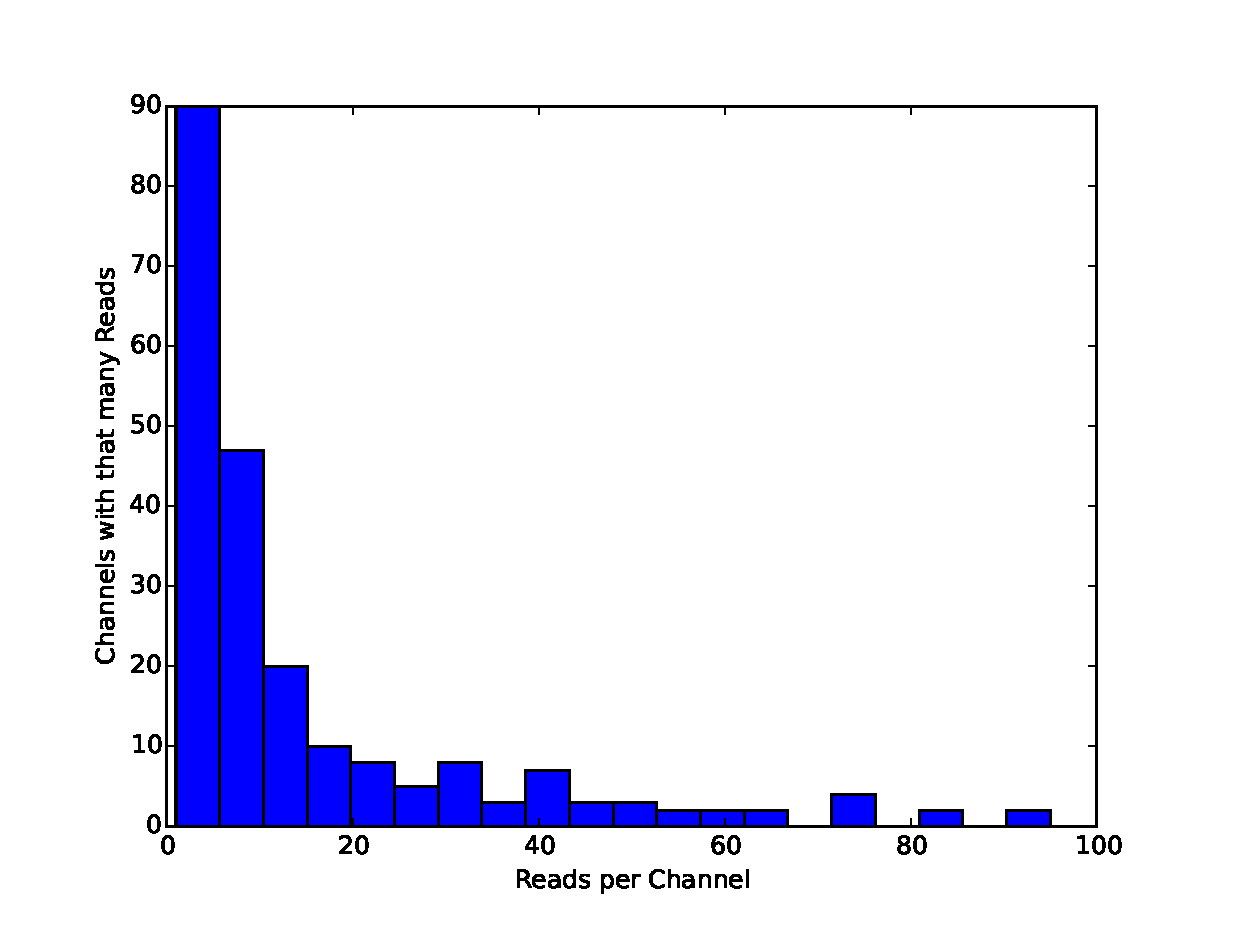
\includegraphics[width=2.5in]{part2hist}
  \vspace{-20pt}
\end{wrapfigure}
218 channels had at least one read. 
The average channel had 14.8 reads. 
Channel 212 had 95 reads, which was the most.

Just for fun, here's a histogram of reads per channel\\
\section*{Problem 3}
\begin{tabular}{cc}
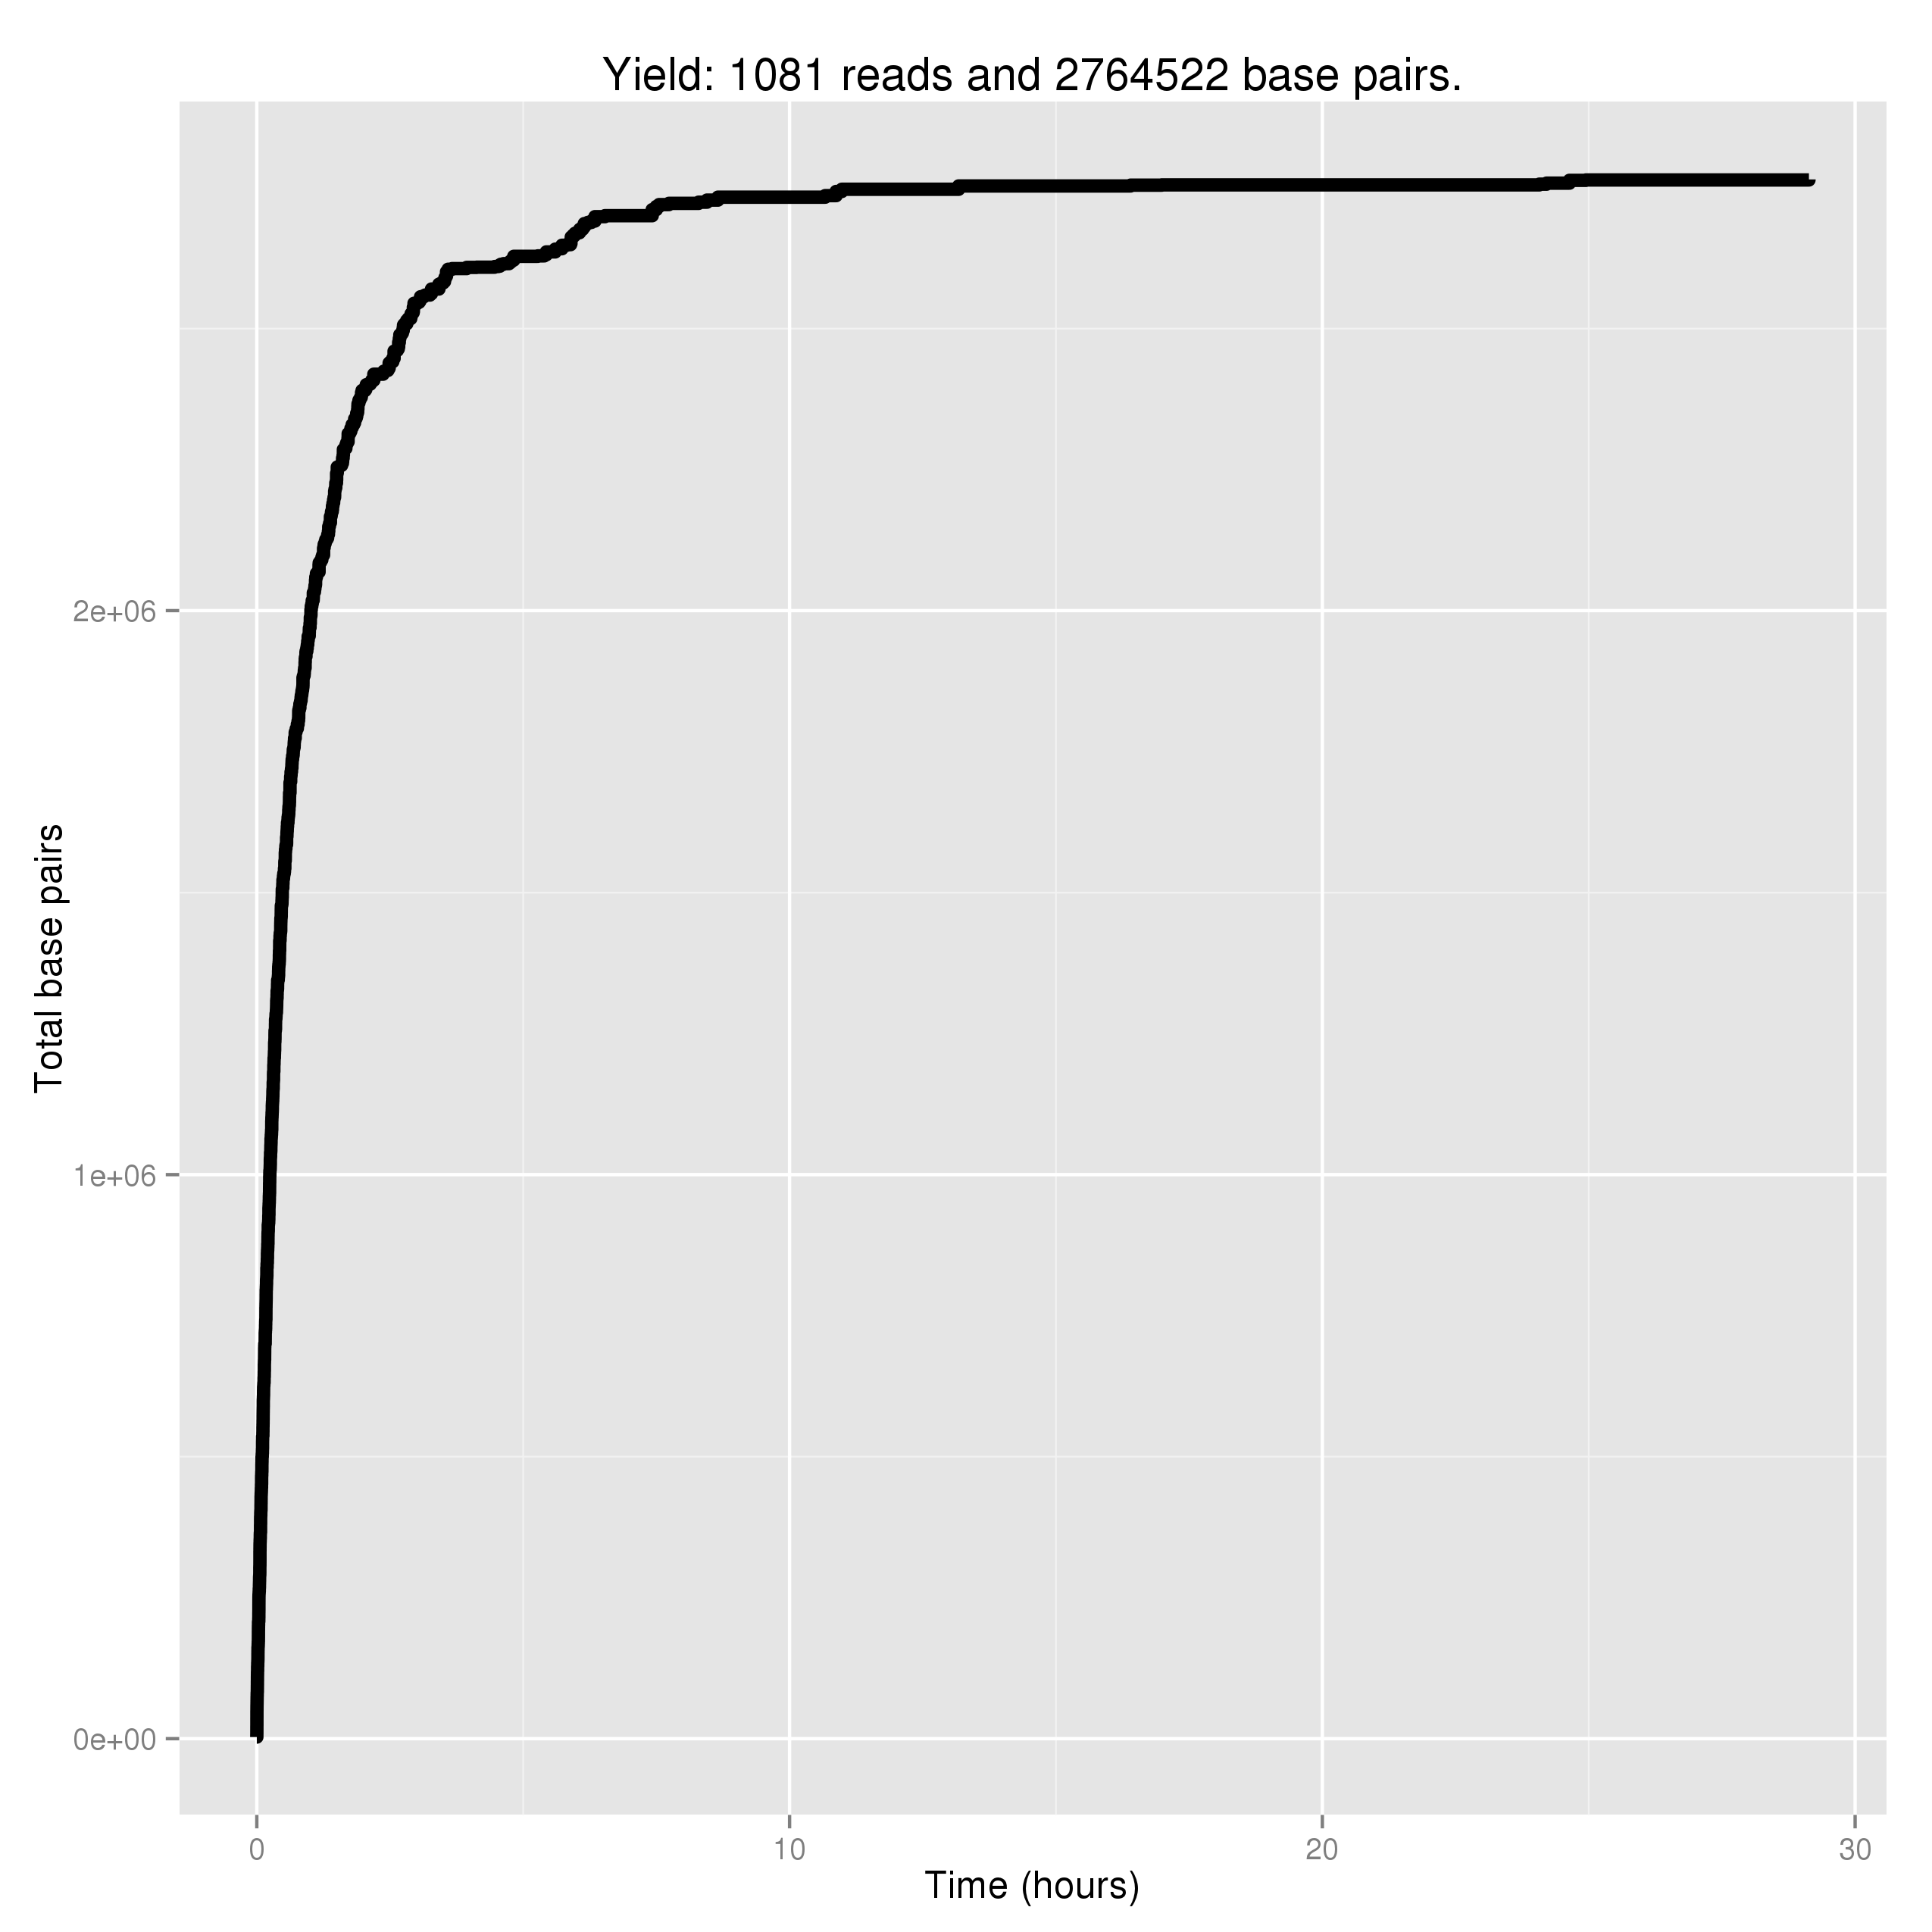
\includegraphics[width=.48\textwidth]{cumnucpass}
&
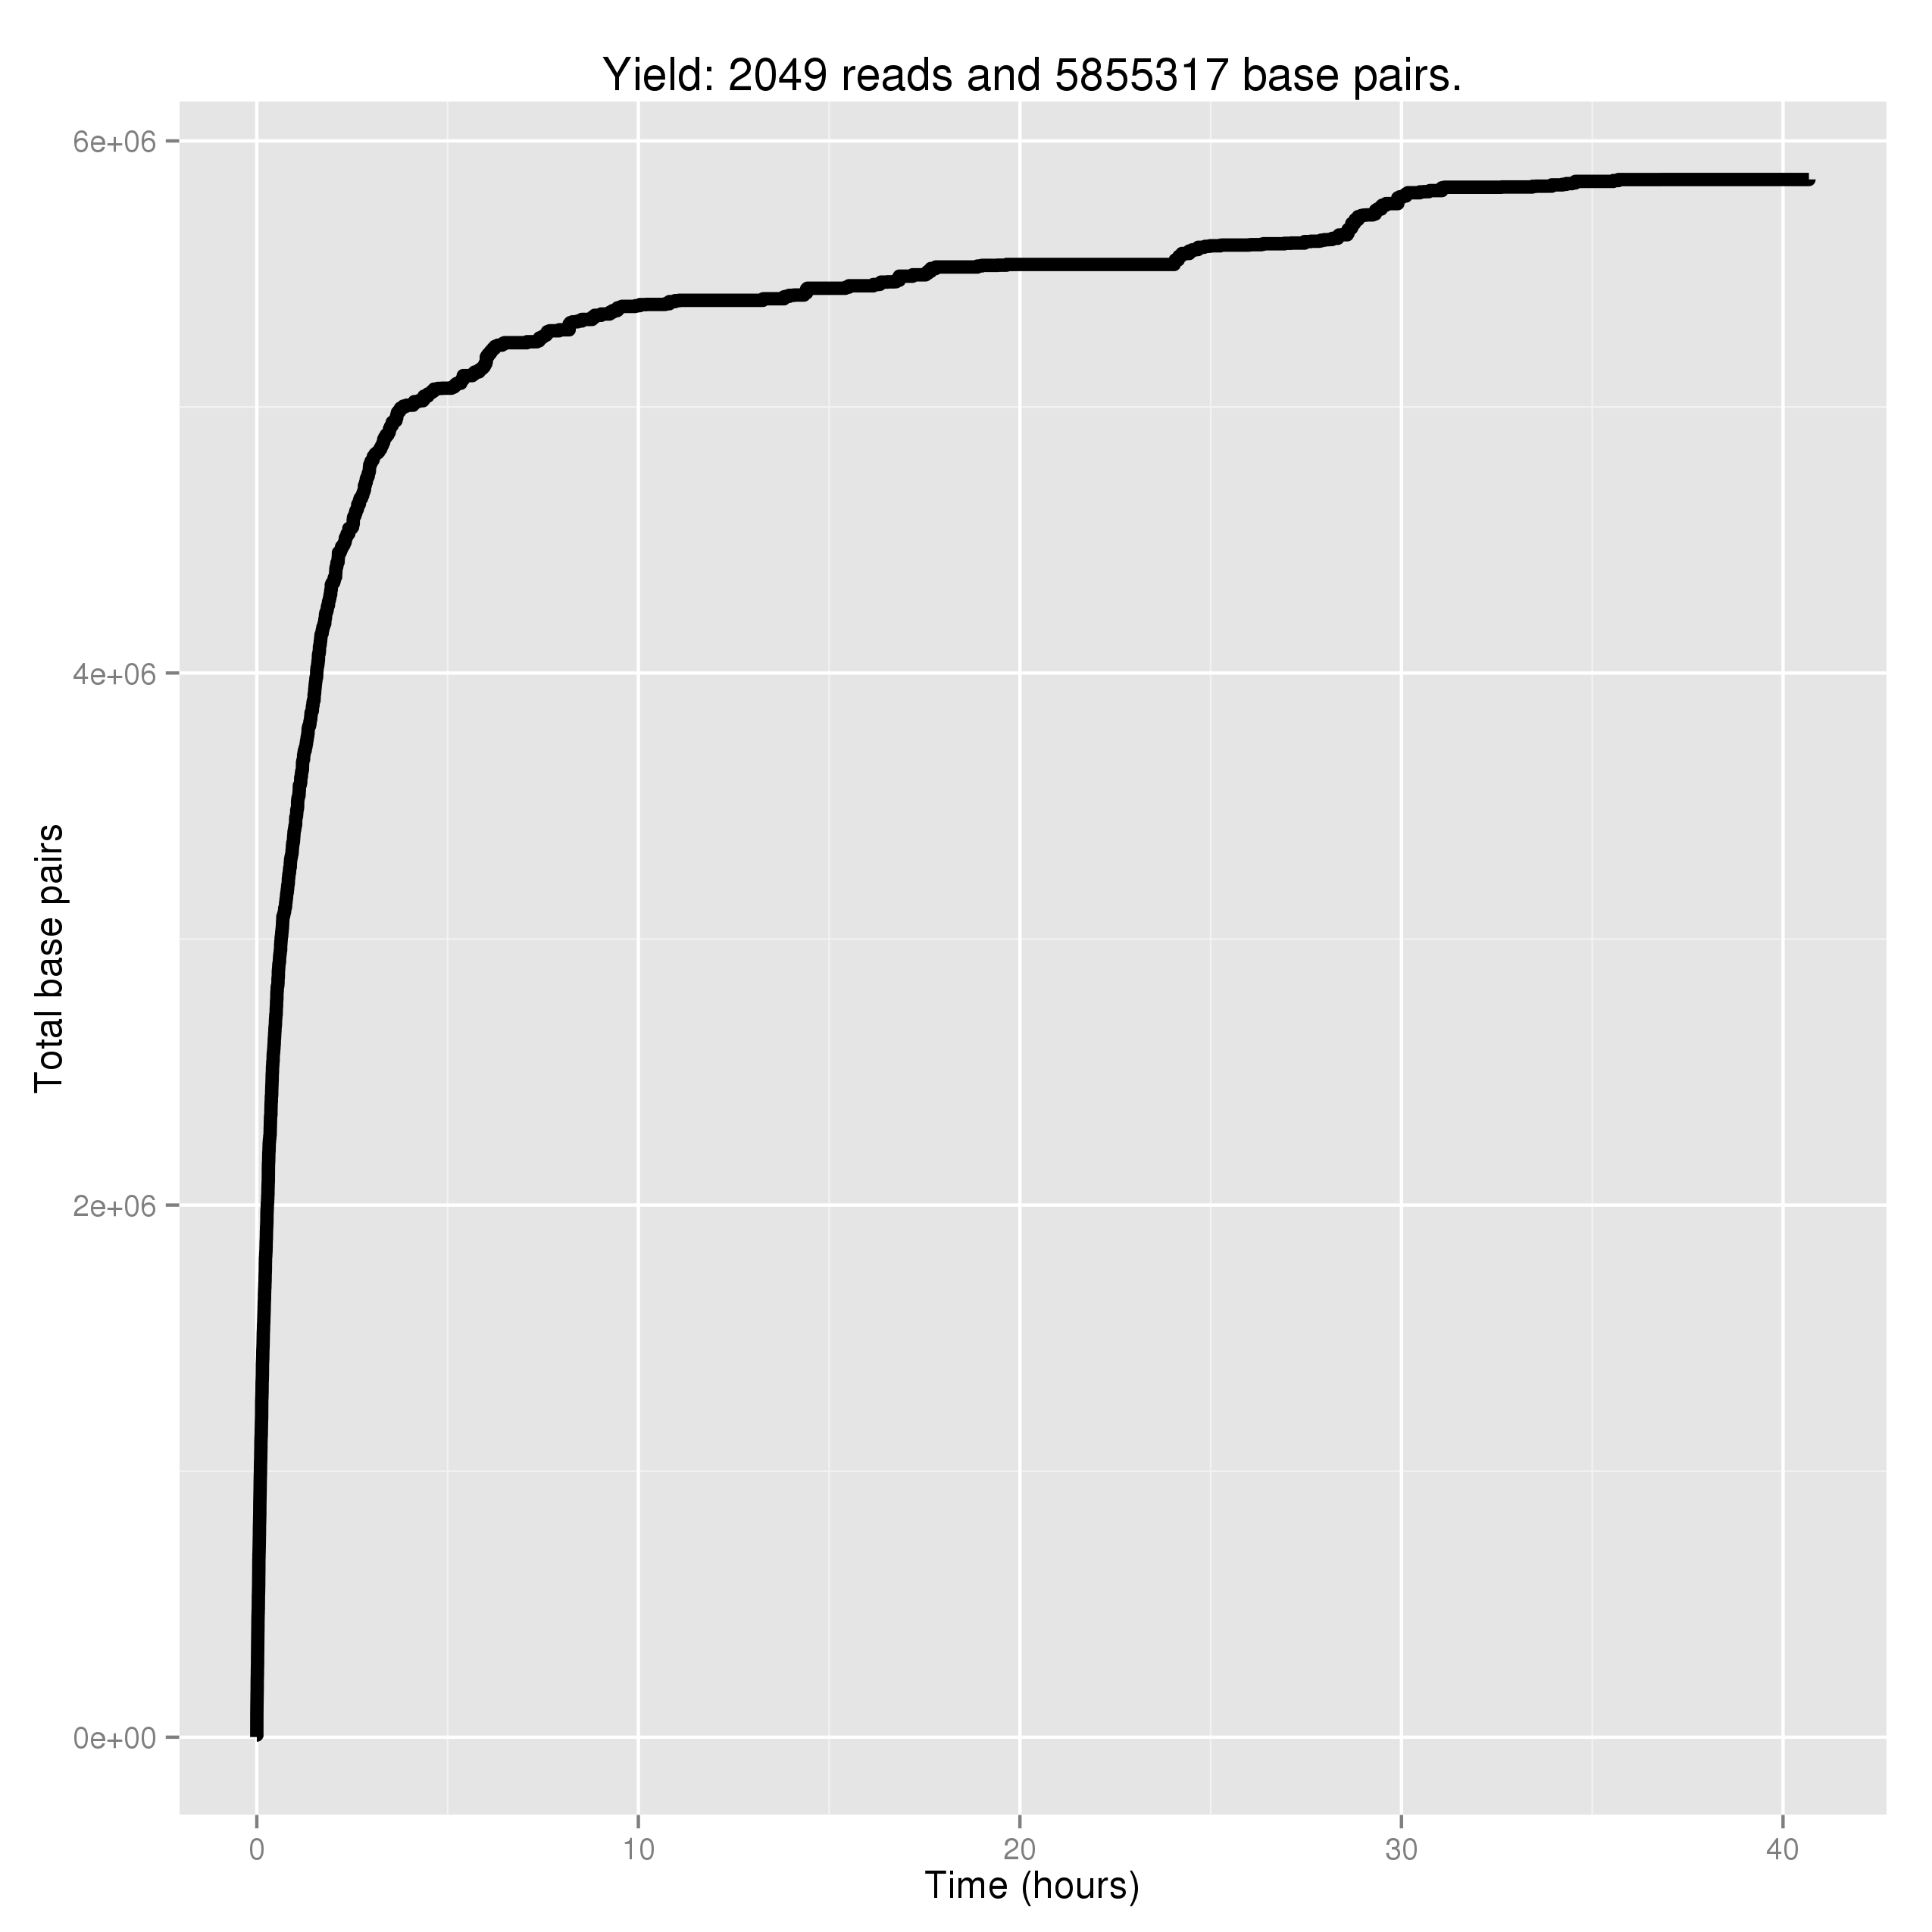
\includegraphics[width=.48\textwidth]{cumnucfail}
\\
Passed Reads
&
Failed Reads
\end{tabular}
\section*{Problem 4}


Let us zoom in a little on the previous graphes: 


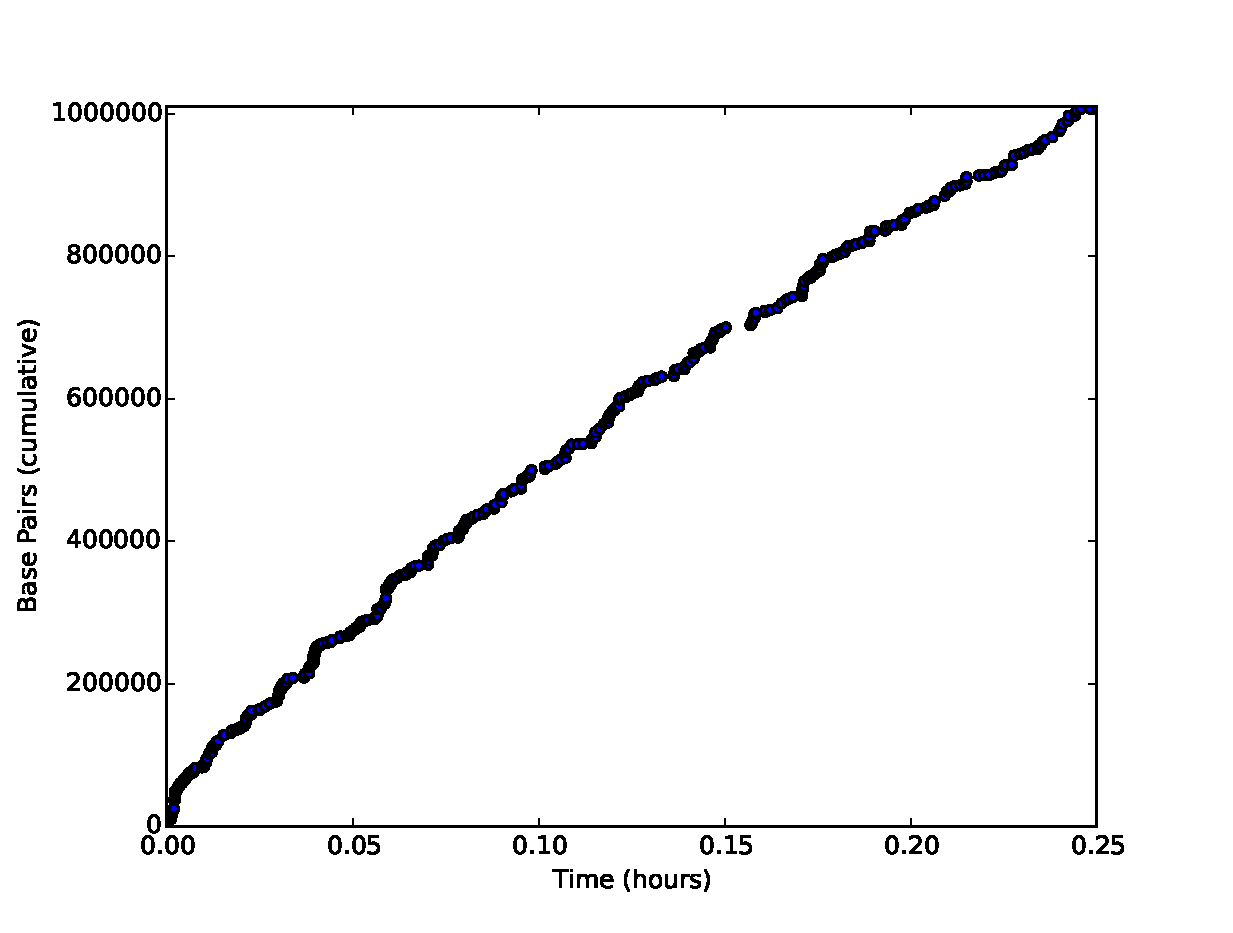
\includegraphics[width=0.48\textwidth]{q4qh}
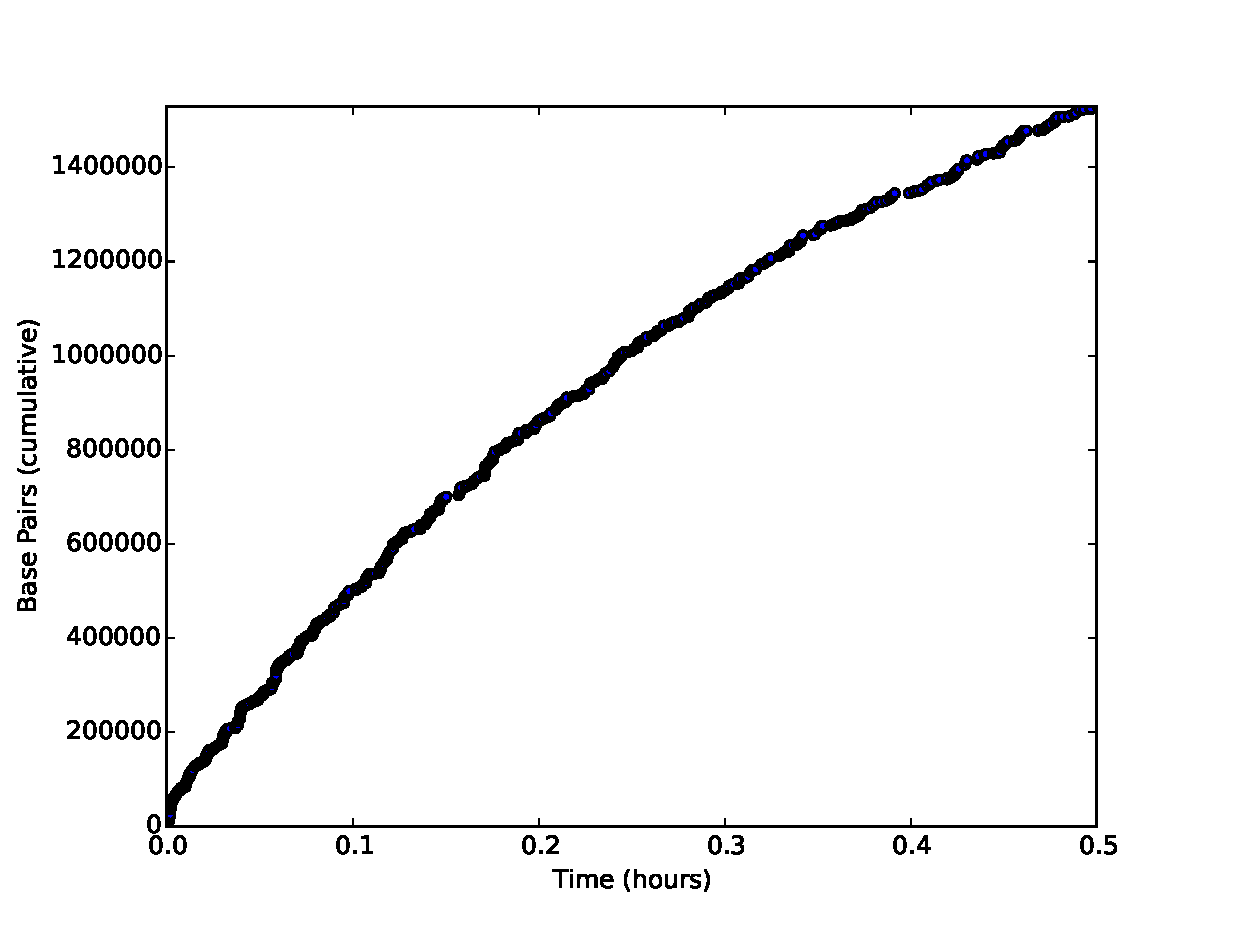
\includegraphics[width=0.48\textwidth]{q4hh}

The first quarter hour appears linear, but the first half hour does not.

To estimate the amout of time needed to sequence the human genome once, 
we used data from the first quarter hour due to its linearity.  We hypothesize 
that the change in sequencing rate is due to a decrease in the molar concentration 
of DNA, and therefore the rate at which a DNA molecule encounters a given pore is 
rate-limiting, rather than a decrease in the effeciecy of the MinION.  Therefore, 
in our calculation, we made the assumption that DNA concentration does not change 
over time and there is only one copy of the genome present to avoid sequencing 
$>$ 1x coverage. 


Over the first half hour, the rate was 1121.4 base pairs per second.  Therefore, to handle the 3 billion base pairs of the human genome would take 743.1 hours.
\section*{Problem 5}
\subsection*{Passed 2D Reads}
Mean Quality Score=10.3775\\  Std. Dev.=1.83151\\ n=2764522\\

\subsection*{Failed 2D Reads}
Mean Quality Score=9.48623\\  Std. Dev.=2.06174\\ n=1417759\\

\subsection*{T-test comparison}
T-Statistic=451.124\\
P-Value=0


The P-value was confirmed to be returned as 0 from Python/numpy.
We believe that the true value is above 0 but beneath the lowest threshold of Python's float value (2.2250738585072014e-308).

\subsection*{Passed 2D Reads - First Hour}
Mean Quality Score=10.3668\\  Std. Dev.=1.82208\\ n=1970130\\
Median=10

\subsection*{Passed 2D Reads - Last Hour}
Mean Quality Score=11.5651\\  Std. Dev.=2.12032\\ n=968\\
Median=11

The quality of the reads does not appear to have degraded over the timespan of the sequencing
(on the contrary, there is a slight increase).
\section*{Problem 6}
\subsection*{1D reads}

        The following histograms show the length distribution of 1D reads (both template and complement) for passes and fails.

        \begin{tabular}{cc}
          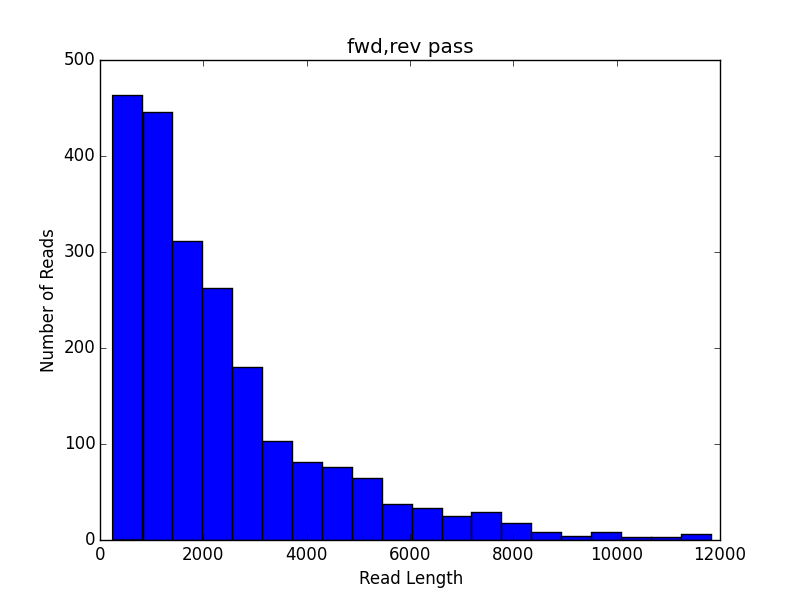
\includegraphics[width=.48\textwidth]{1Dpasses}
          &
          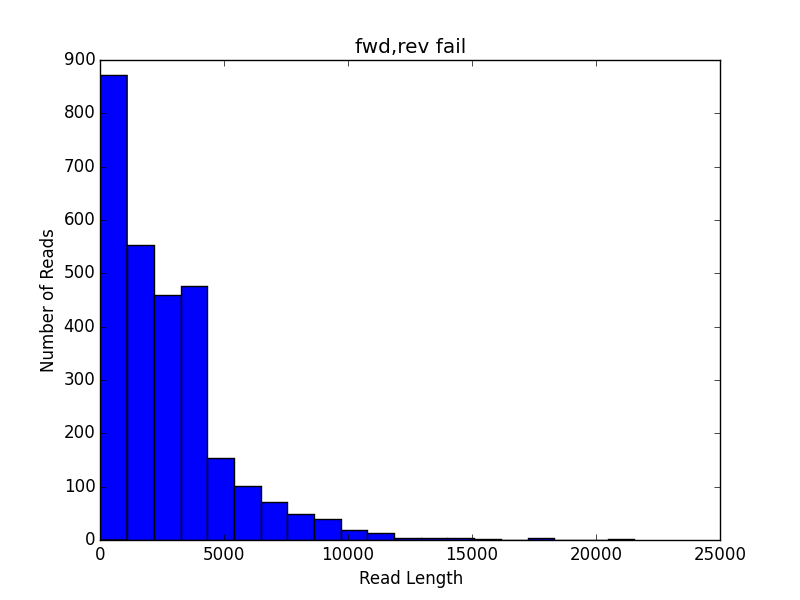
\includegraphics[width=.48\textwidth]{1Dfailures}
          \\
          Passed Reads
          &
          Failed Reads
        \end{tabular}
        

\subsection*{2D reads}

        The following histograms show the length distribution of 2D reads for passes and fails.

        
        \begin{tabular}{cc}
          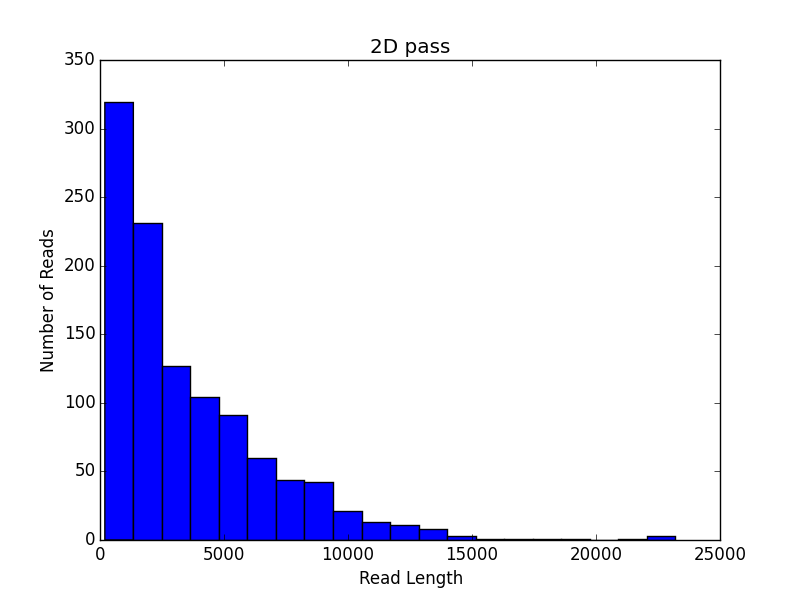
\includegraphics[width=.48\textwidth]{2Dpasses}
          &
          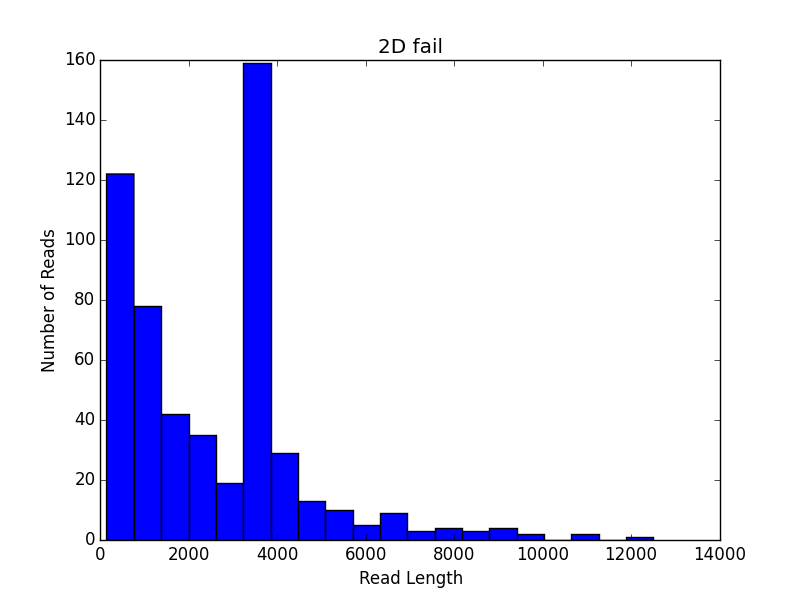
\includegraphics[width=.48\textwidth]{2Dfailures}
          \\
          Passed Reads
          &
          Failed Reads
        \end{tabular}

        
\subsection*{1D and 2D reads}

        The following histogramss show the cumulative length distribution of both 1D and 2D reads for passes and fails.

        
        \begin{tabular}{cc}
          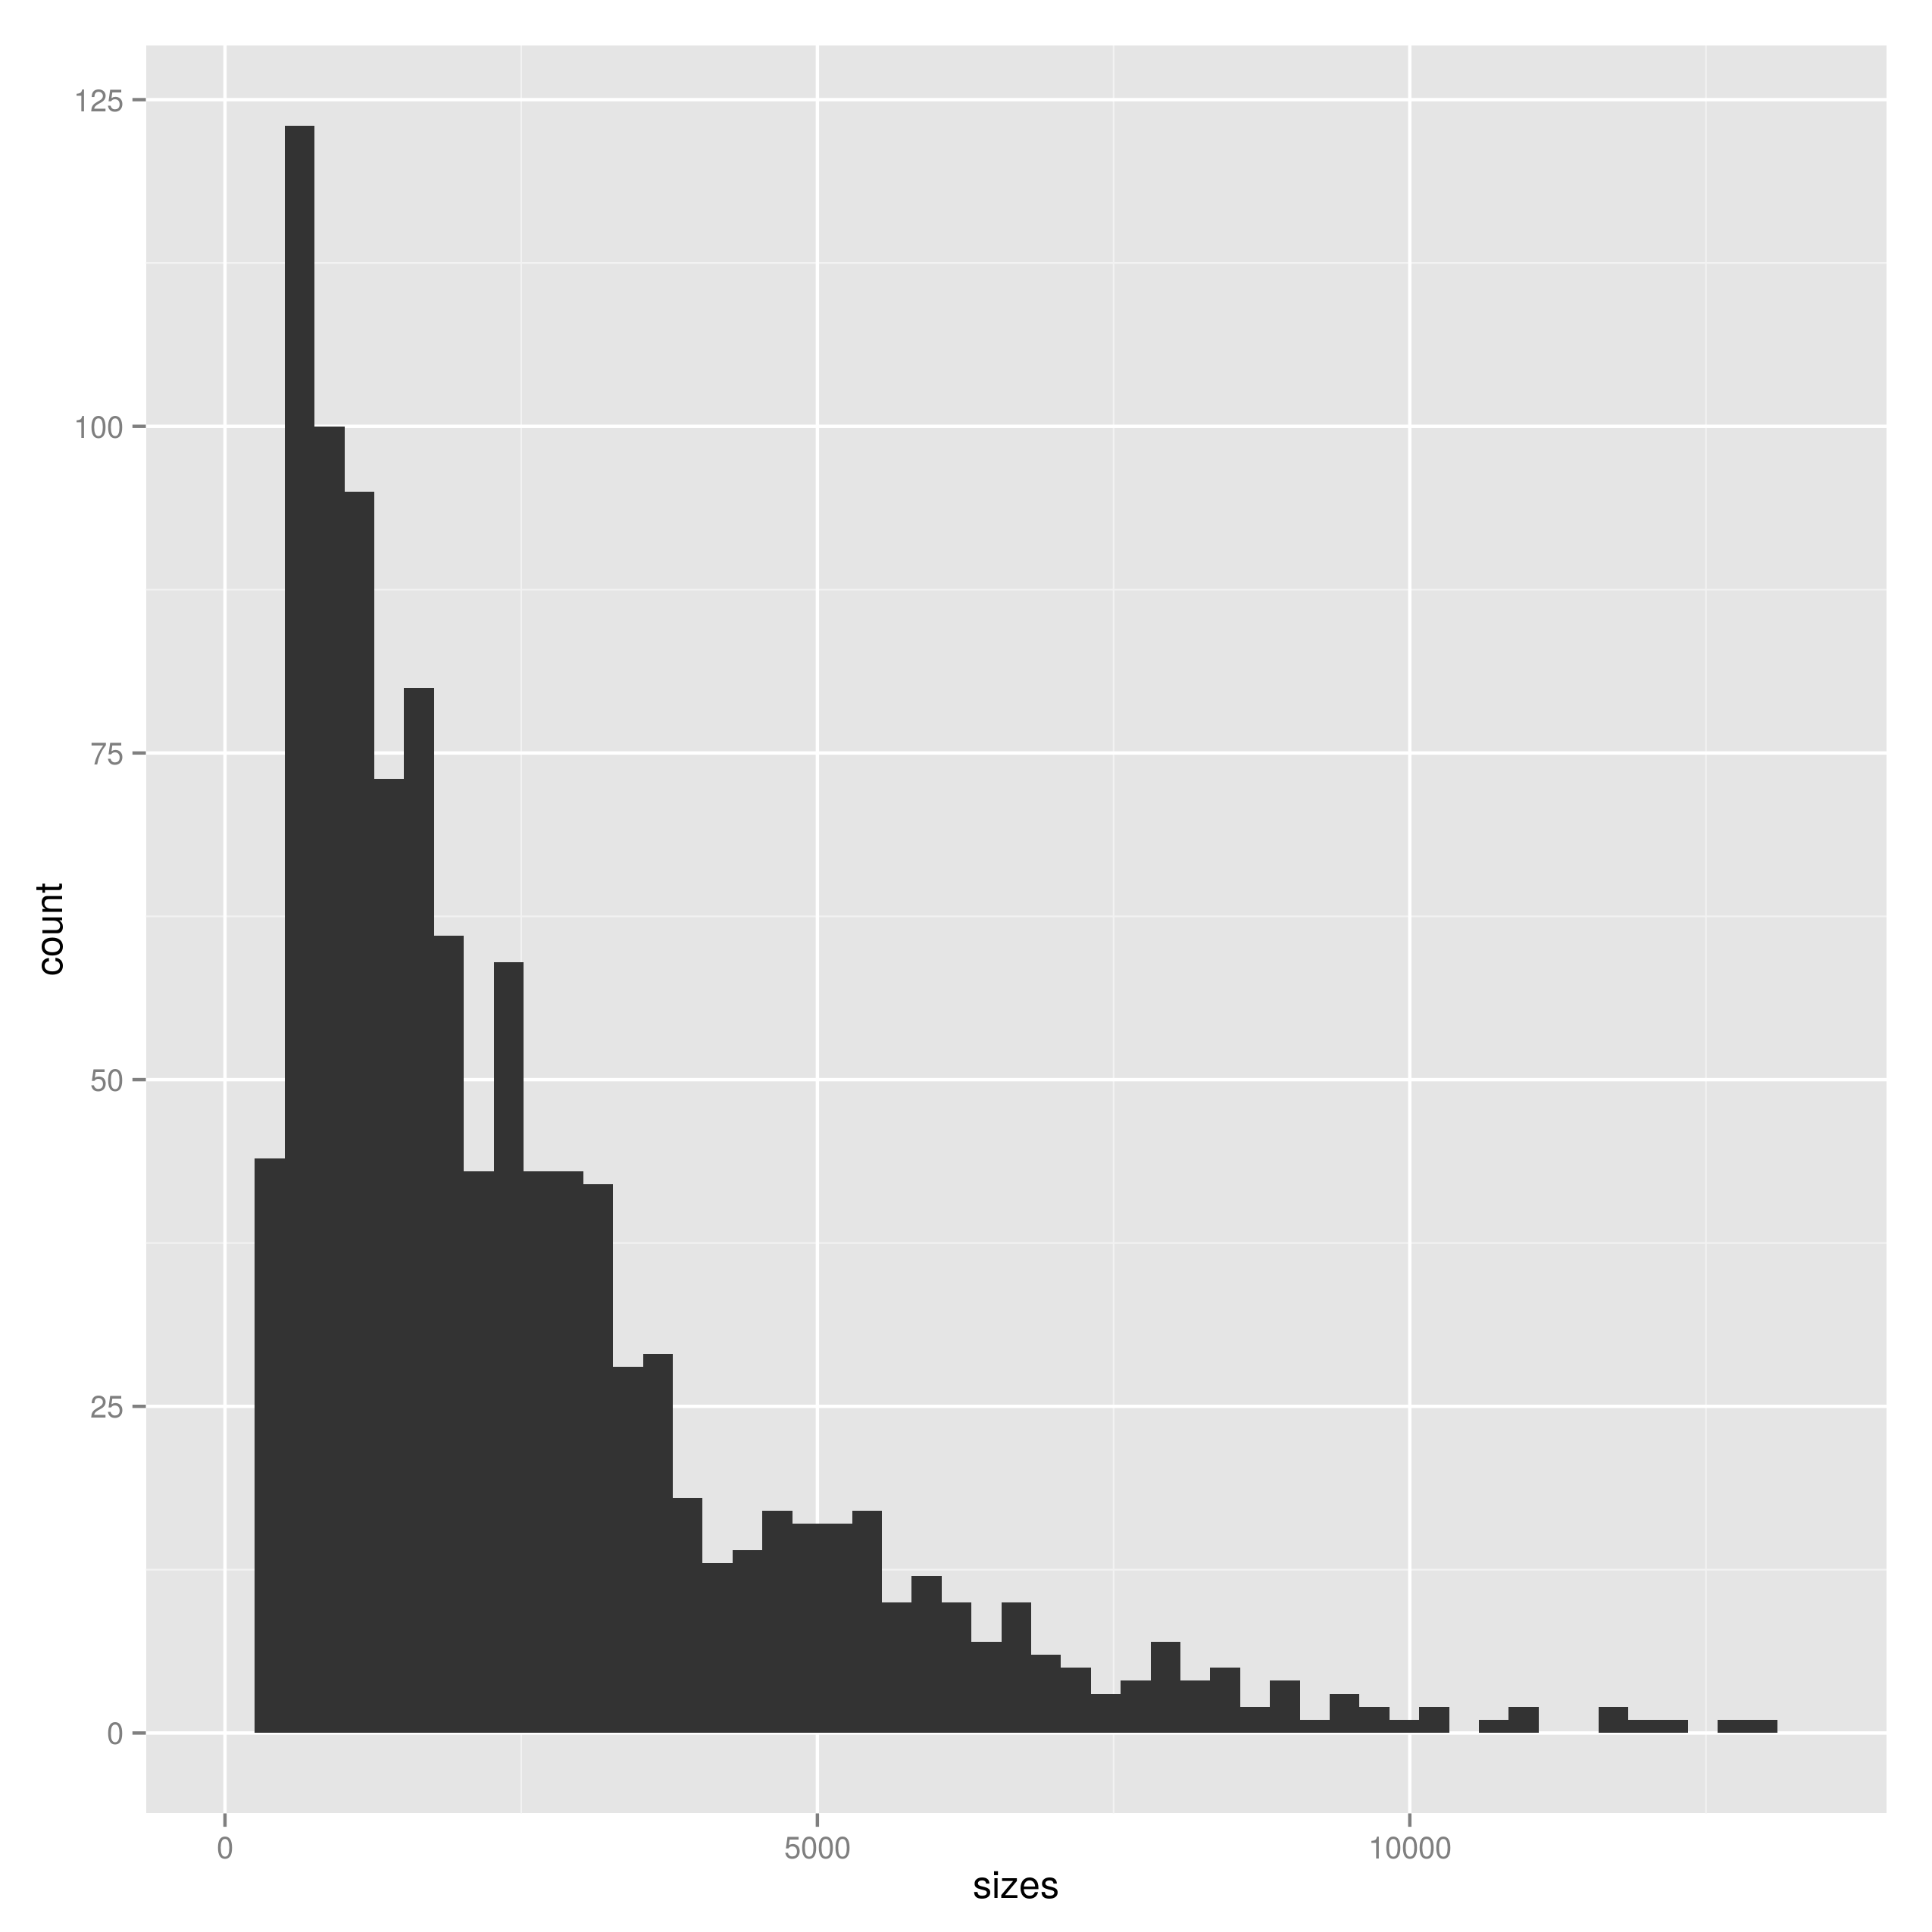
\includegraphics[width=.48\textwidth]{histallpass}
          &
          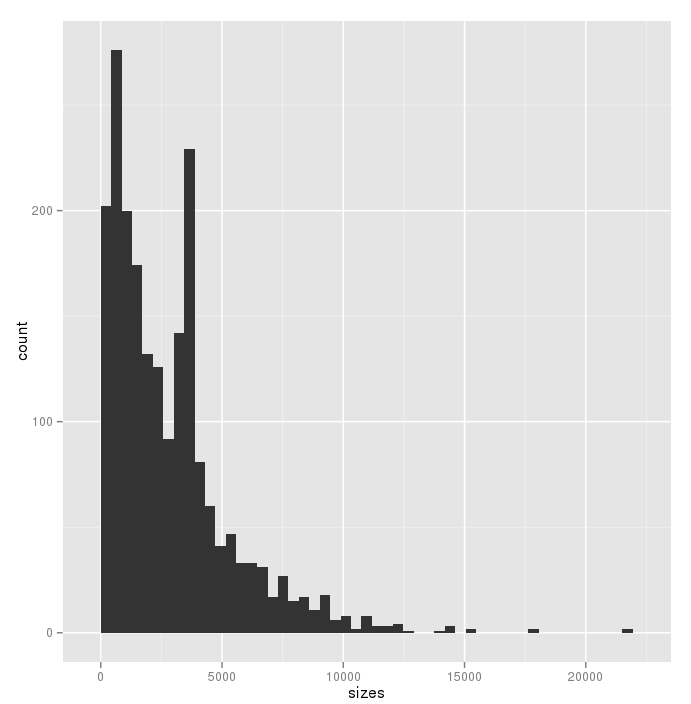
\includegraphics[width=.48\textwidth]{histallfail}
          \\
          Passed Reads
          &
          Failed Reads
        \end{tabular}
\section*{Problem 7}

LONGEST TEMPLATE READ\\
From file: MINION02\_4teamawesome\_2446\_1\_ch312\_file44\_strand.fast5\\
Number of nucleotides: 11820\\

LONGEST COMPLEMENT READ\\
From file: MINION02\_4teamawesome\_2446\_1\_ch312\_file44\_strand.fast5\\
Number of nucleotides: 11498\\

LONGEST 2D READ\\
From file: MINION02\_4teamawesome\_2446\_1\_ch312\_file44\_strand.fast5\\
Number of nucleotides: 12916\\
\section*{Problem 8}
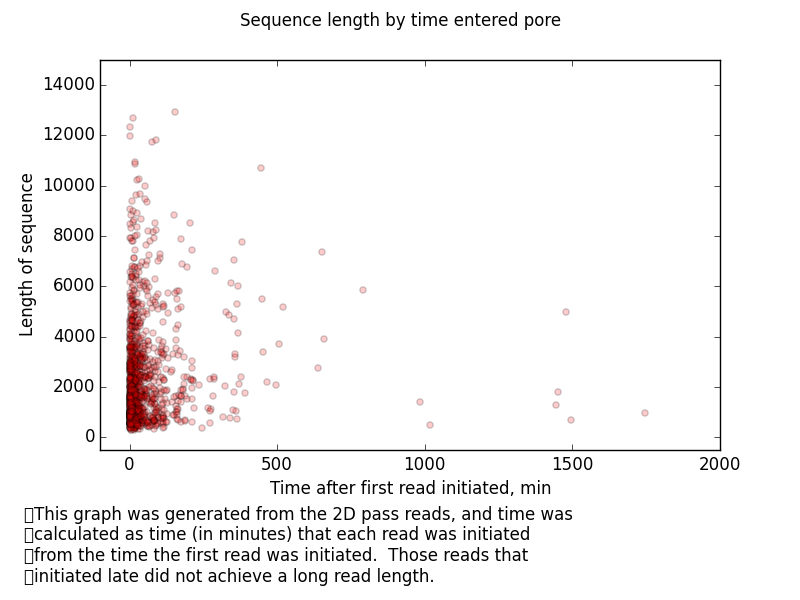
\includegraphics[width=\textwidth]{q8}
\section*{Problem 9}
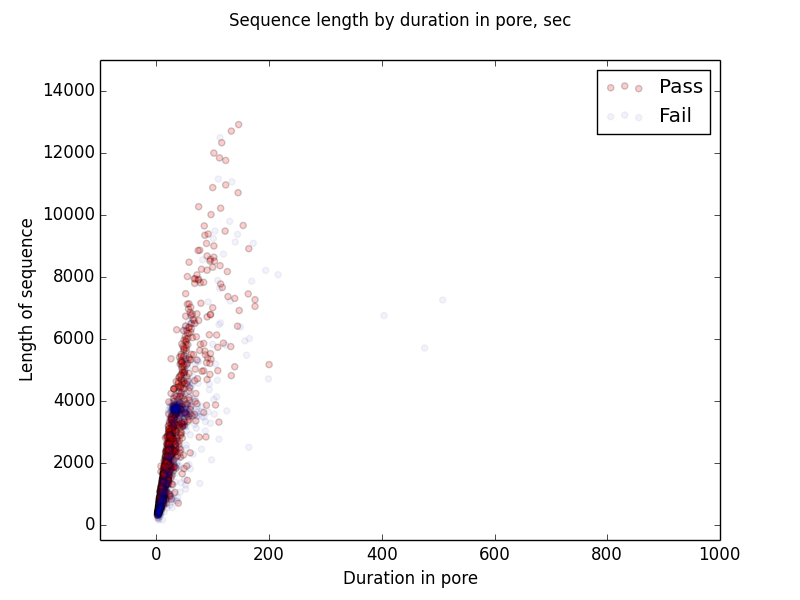
\includegraphics[width=\textwidth]{q9}
\section*{Problem 10}
Computing nucleotide composition of passed reads...\\
Failed reads \%Composition\\
\% A: 26.8544936058\\
\% C: 22.6248607838\\
\% T: 26.8972371186\\
\% G: 23.6234084919\\
\\
Computing nucleotide composition of failed reads...\\
Passed reads \%Composition\\
\% A: 27.8932849874\\
\% C: 21.7440845108\\
\% T: 27.990263778\\
\% G: 22.3723667238\\
\section*{Problem 11}
\subsection*{Simple Model}

        The simplest possible model is the one in which the number of nucleotides determines the read duration,
        possibly with some constant term for getting started.  To consider this, we start with a scatterplot of
        bases against time with a linear fit.

        \begin{centering}
        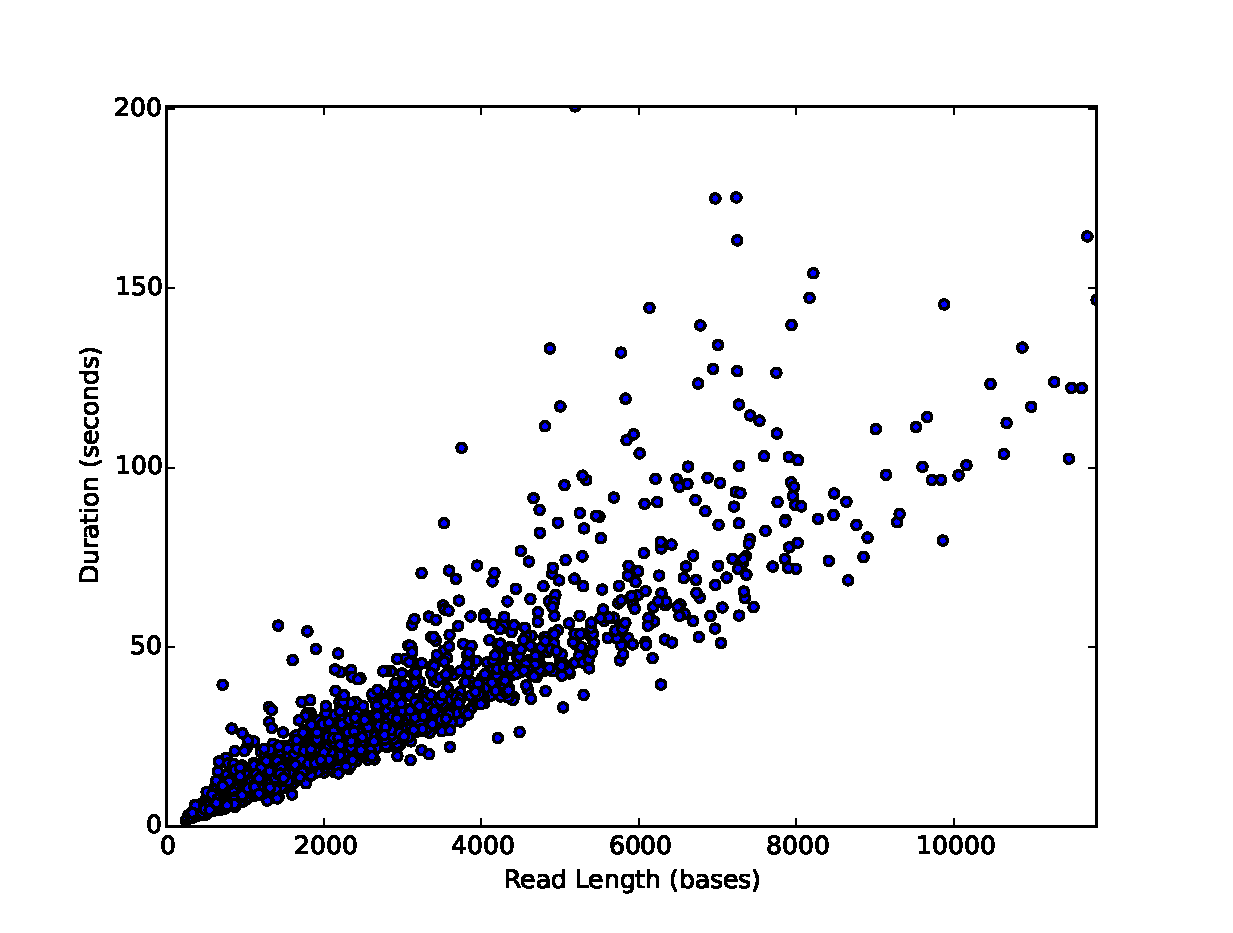
\includegraphics[width=\textwidth]{part11scatterbd}
        \end{centering}

        We might be tempted to include a constant term in our fitting, but as should be apparent, it would be
        negative.  How long it would take to sequence an extremely short read is unclear.  Fortunately, there 
        are none in our sample.

        \newpage
        This allows us to construct a trivial (and still pretty effective) model based on a fixed cost per nucleotide.

        Cost per nucleotide: 11.25ms
        
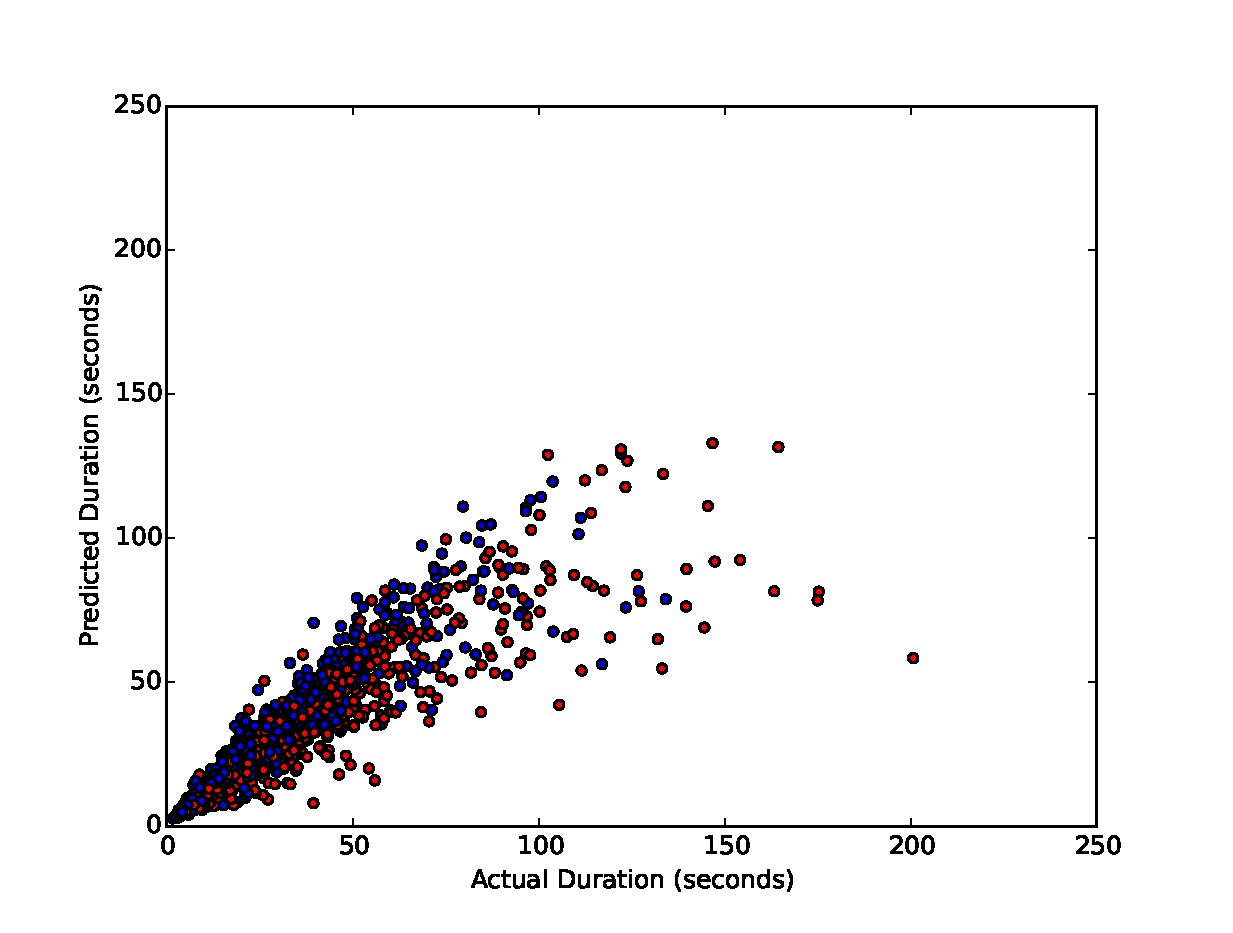
\includegraphics[width=\textwidth]{part11scatter0mer}

$r^2=0.84$


(Red circles are template strand; blue are complement.  There appears to be no significant difference between them.)

\newpage
\subsection*{Nucleotide Model}
A slightly more complex model uses a differend cost for each type of nucleotide: 
A=32ms 
C=-07ms 
G=04ms 
T=12ms 


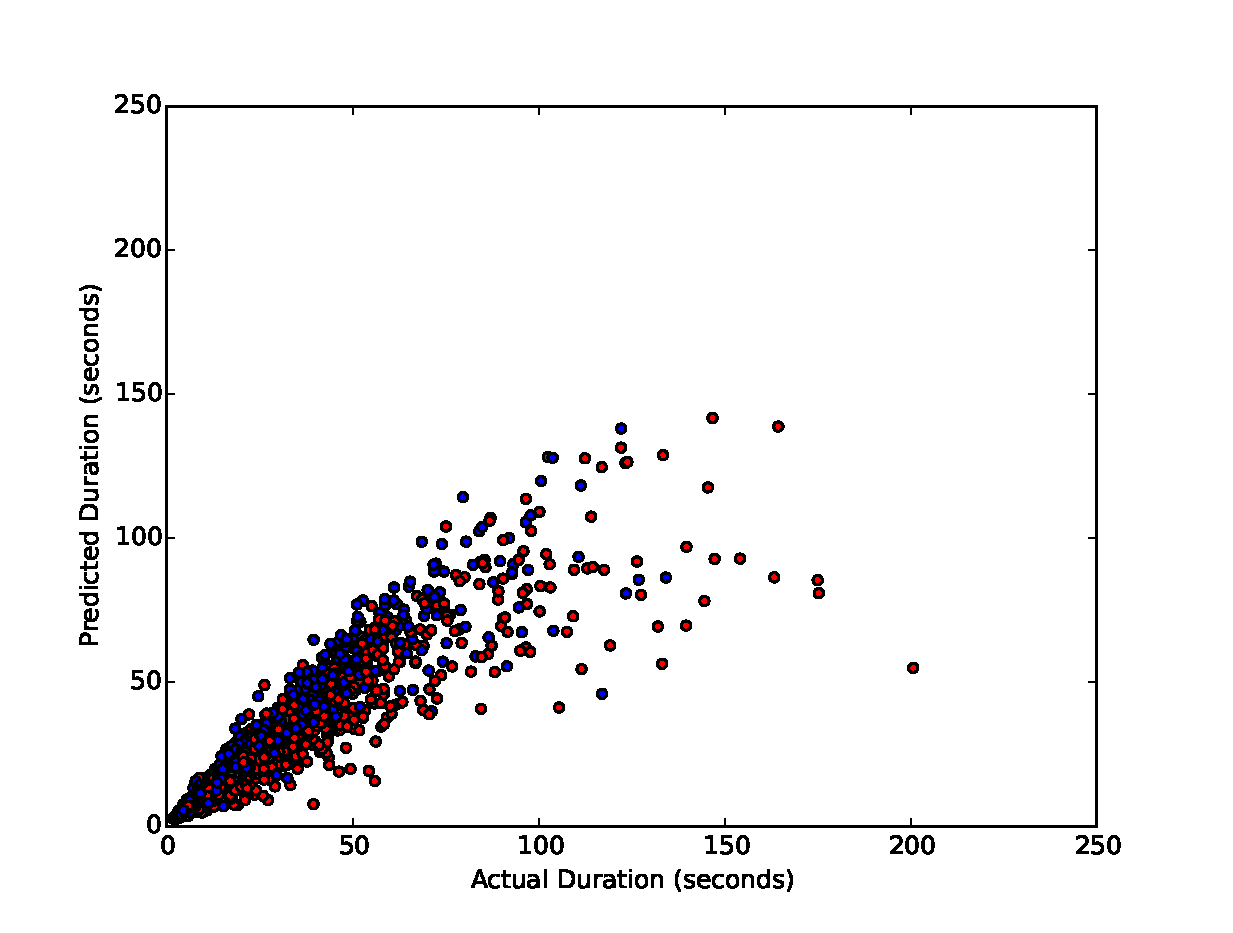
\includegraphics[width=\textwidth]{part11scatter1mer}

$r^2=0.84$


        \newpage
        \subsection*{2mer Model}
        \begin{wrapfigure}{R}{2in}
        \vspace{-50pt}
        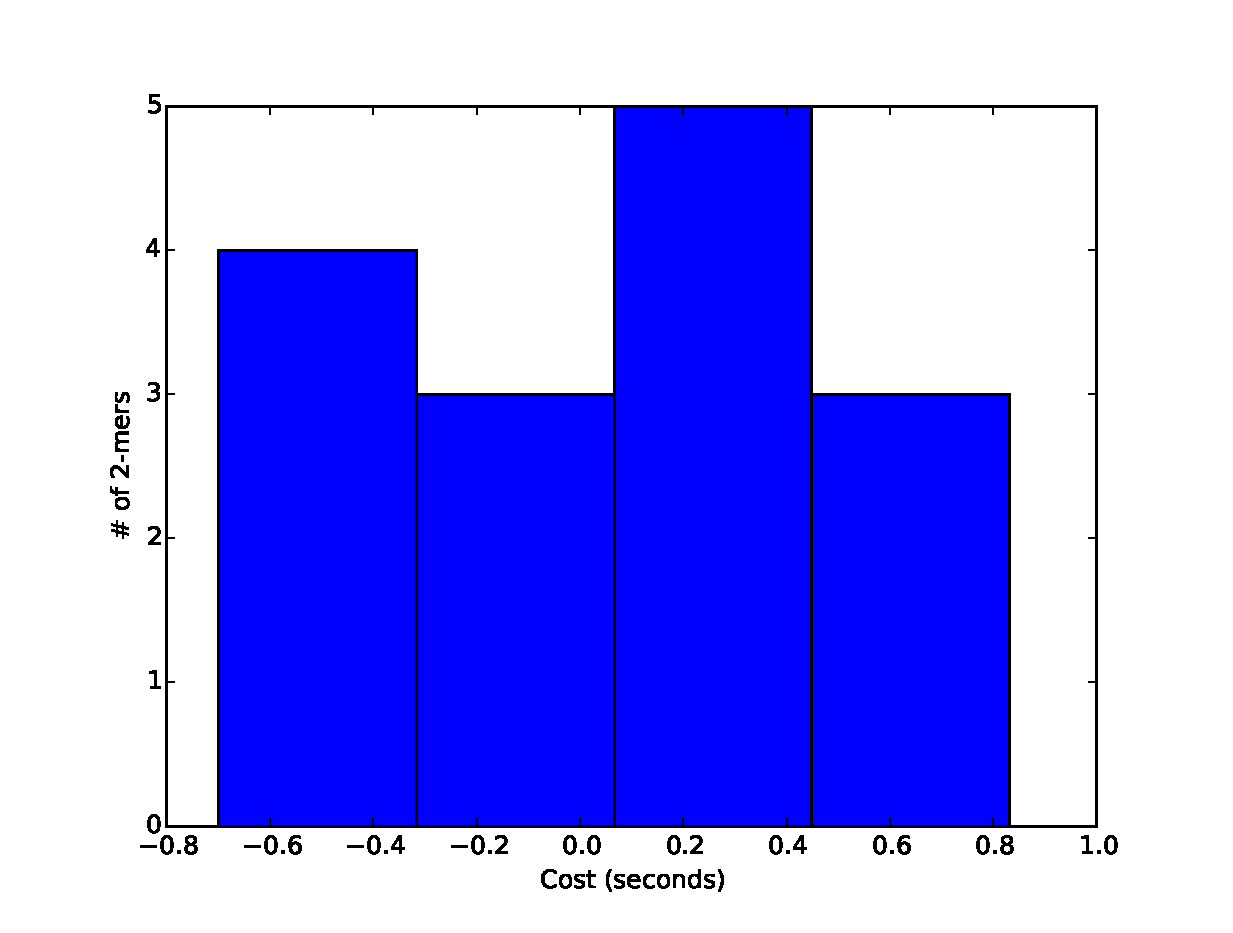
\includegraphics[width=3in]{part11hist2}
        \vspace{-70pt}
        \end{wrapfigure}
        We can use a model in which each the time to extend by one nucleotide is determined by the 2-mer in the middle of the
        pore.  We can not list all the costs, but here's a histogram:

        \vspace{1.5in}

        And here's the resulting predictions:
        
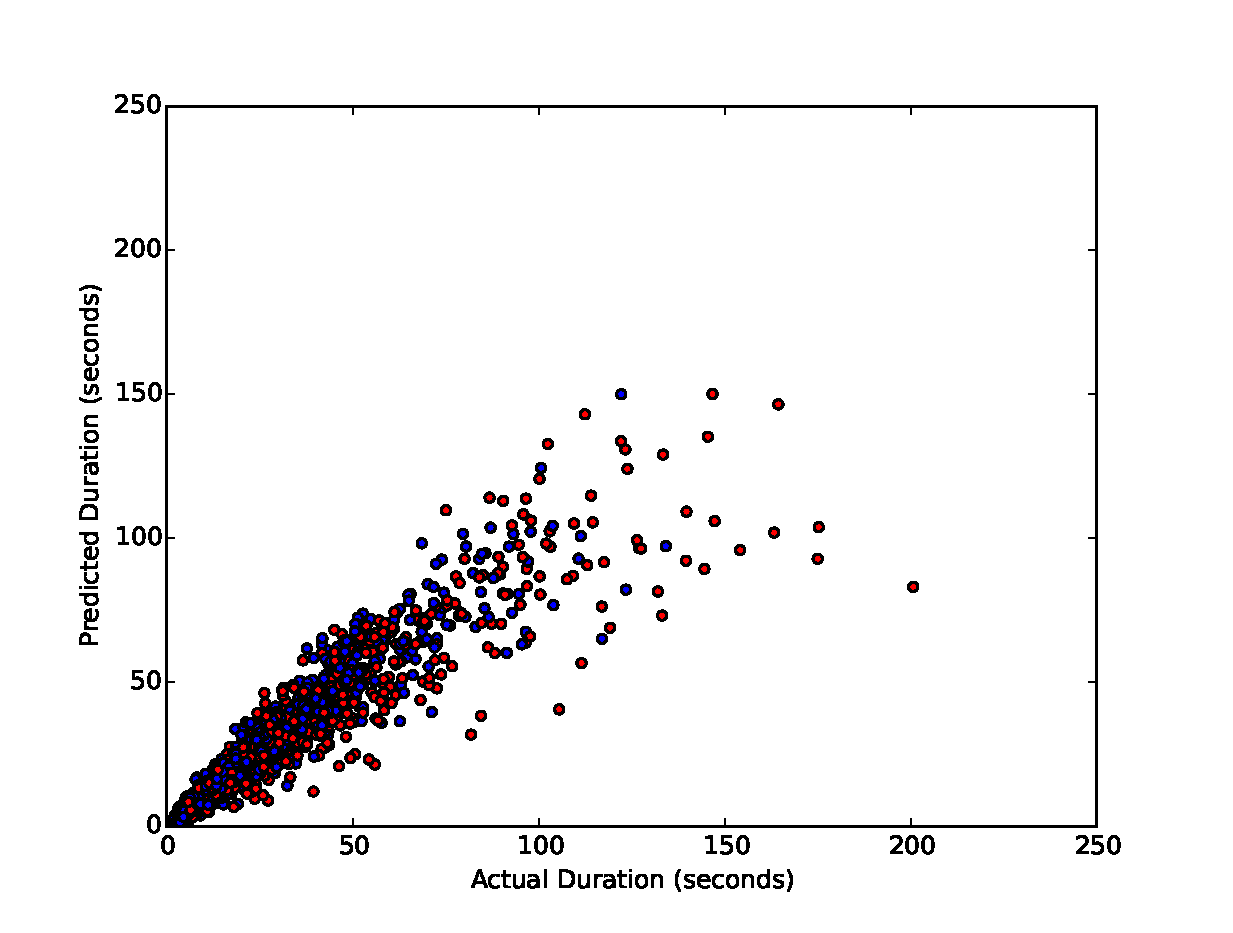
\includegraphics[width=\textwidth]{part11scatter2mer}

$r^2=0.88$


        \newpage
        \subsection*{3mer Model}
        \begin{wrapfigure}{R}{2in}
        \vspace{-50pt}
        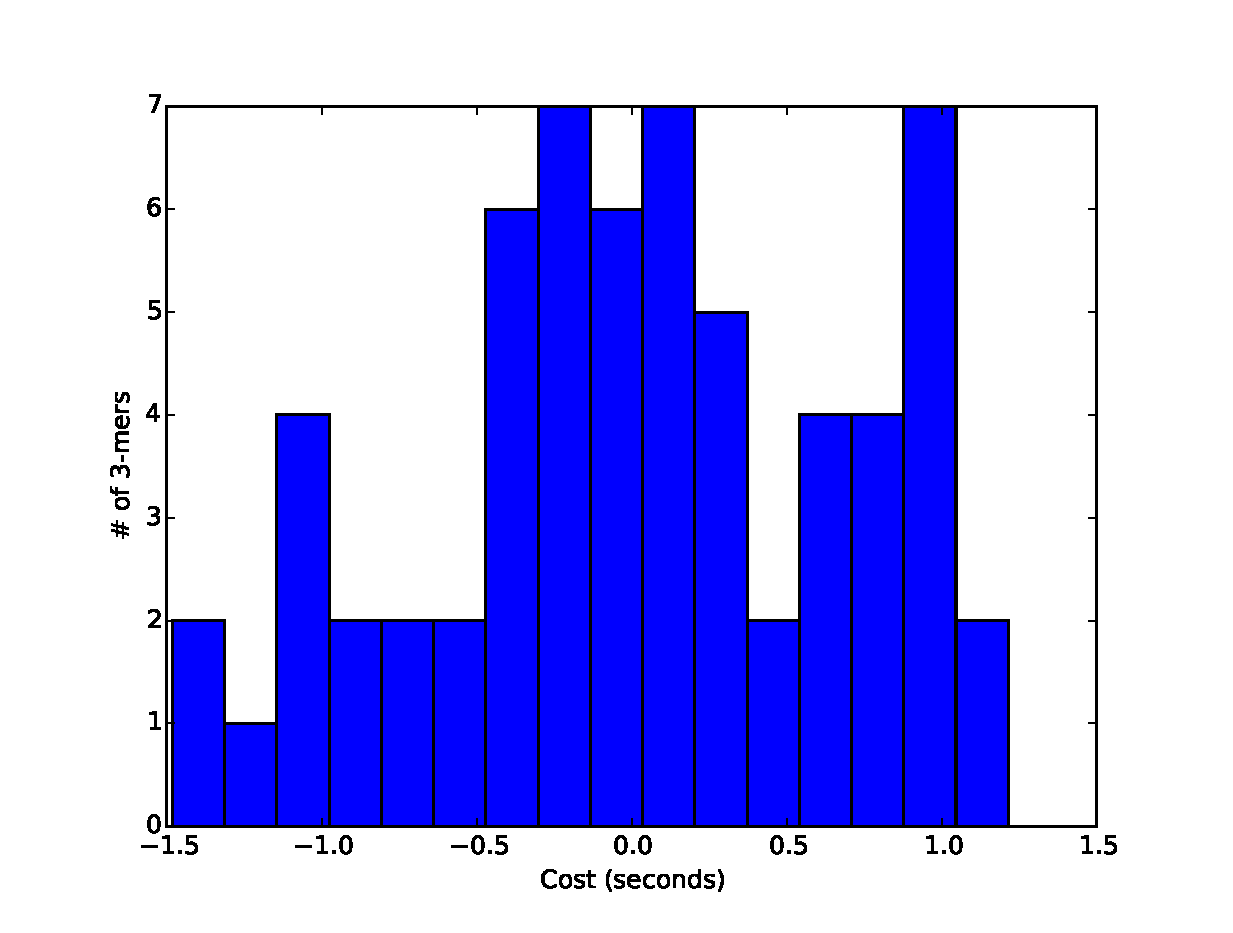
\includegraphics[width=3in]{part11hist3}
        \vspace{-70pt}
        \end{wrapfigure}
        We can use a model in which each the time to extend by one nucleotide is determined by the 3-mer in the middle of the
        pore.  We can not list all the costs, but here's a histogram:

        \vspace{1.5in}

        And here's the resulting predictions:
        
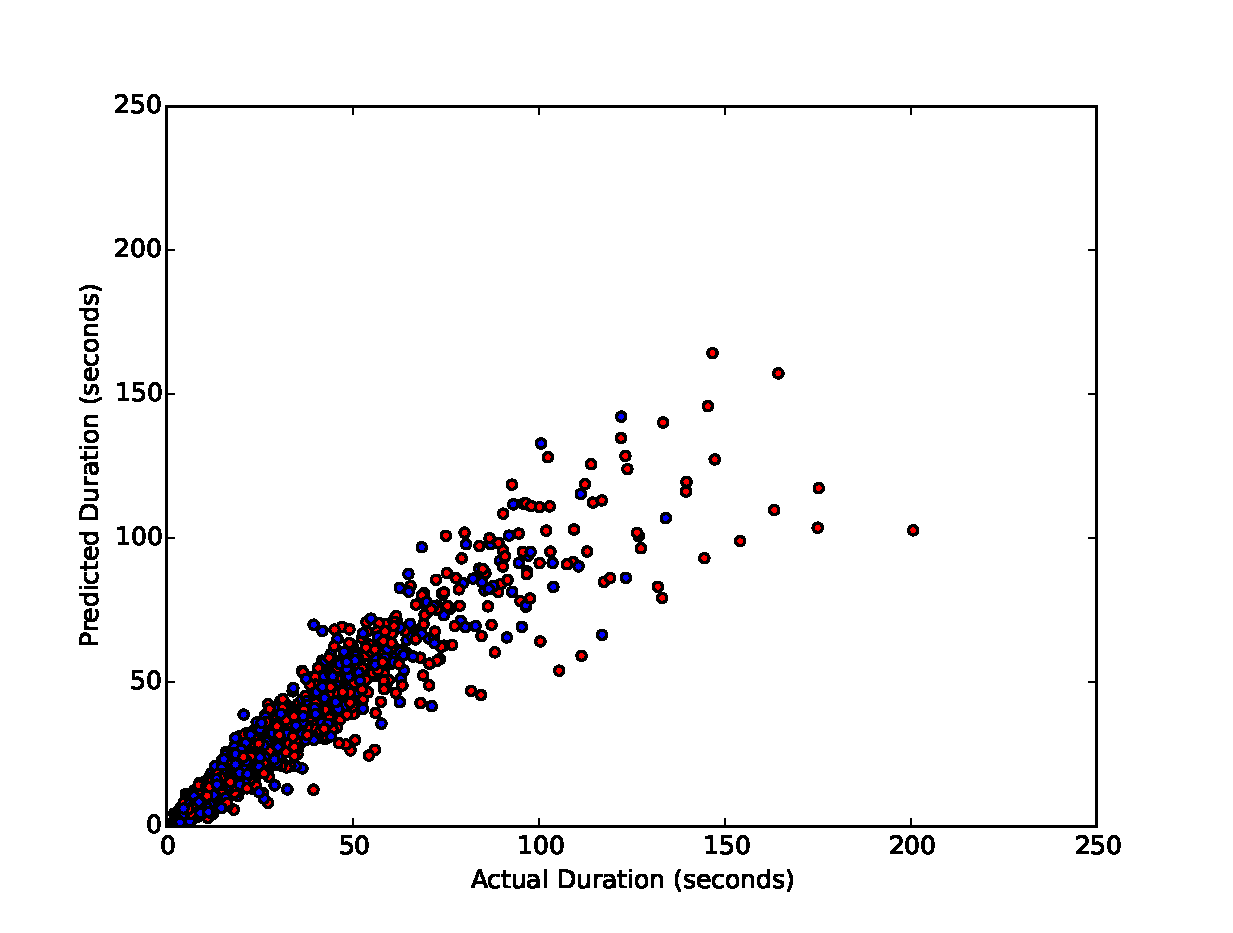
\includegraphics[width=\textwidth]{part11scatter3mer}

$r^2=0.91$


        \newpage
        \subsection*{4mer Model}
        \begin{wrapfigure}{R}{2in}
        \vspace{-50pt}
        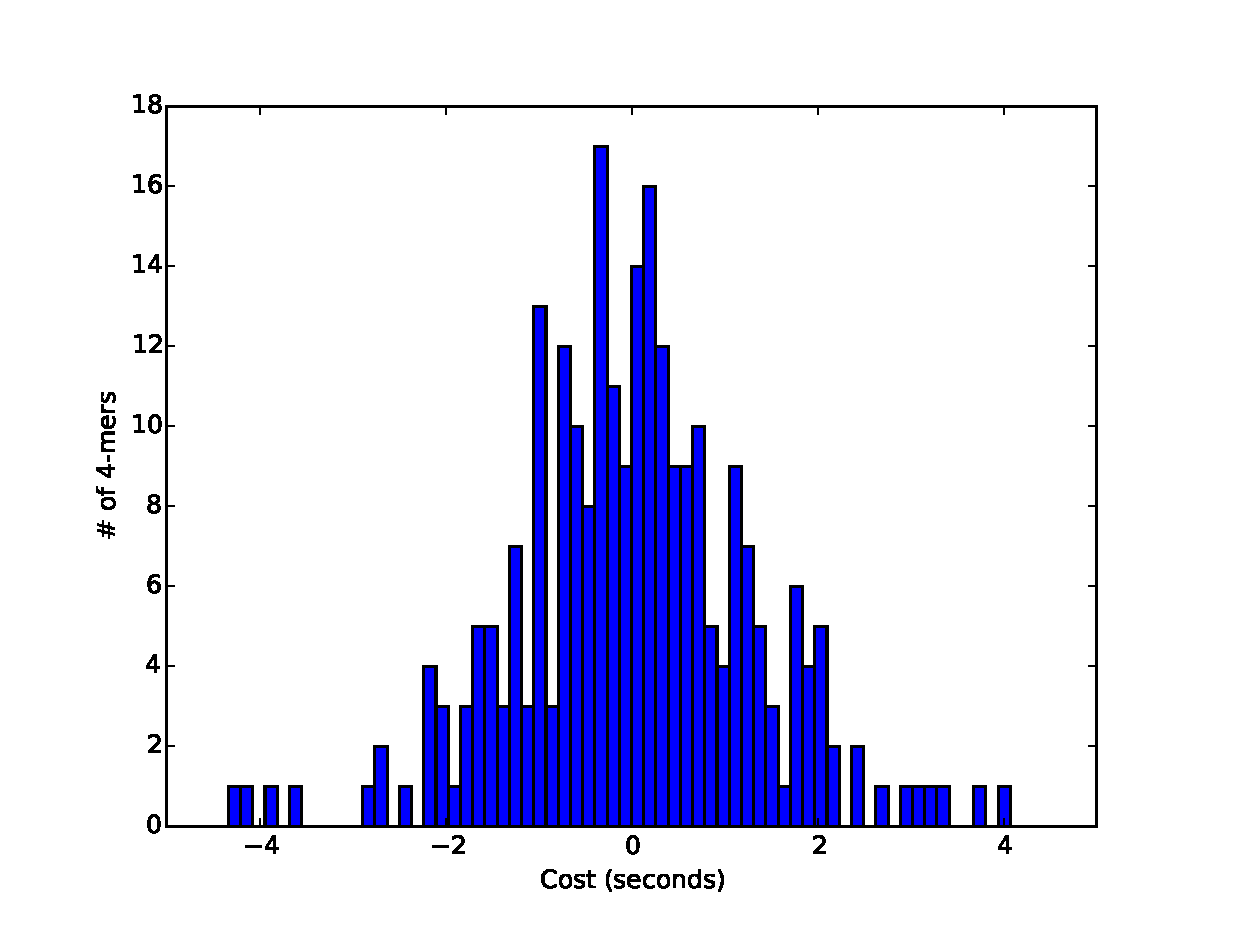
\includegraphics[width=3in]{part11hist4}
        \vspace{-70pt}
        \end{wrapfigure}
        We can use a model in which each the time to extend by one nucleotide is determined by the 4-mer in the middle of the
        pore.  We can not list all the costs, but here's a histogram:

        \vspace{1.5in}

        And here's the resulting predictions:
        
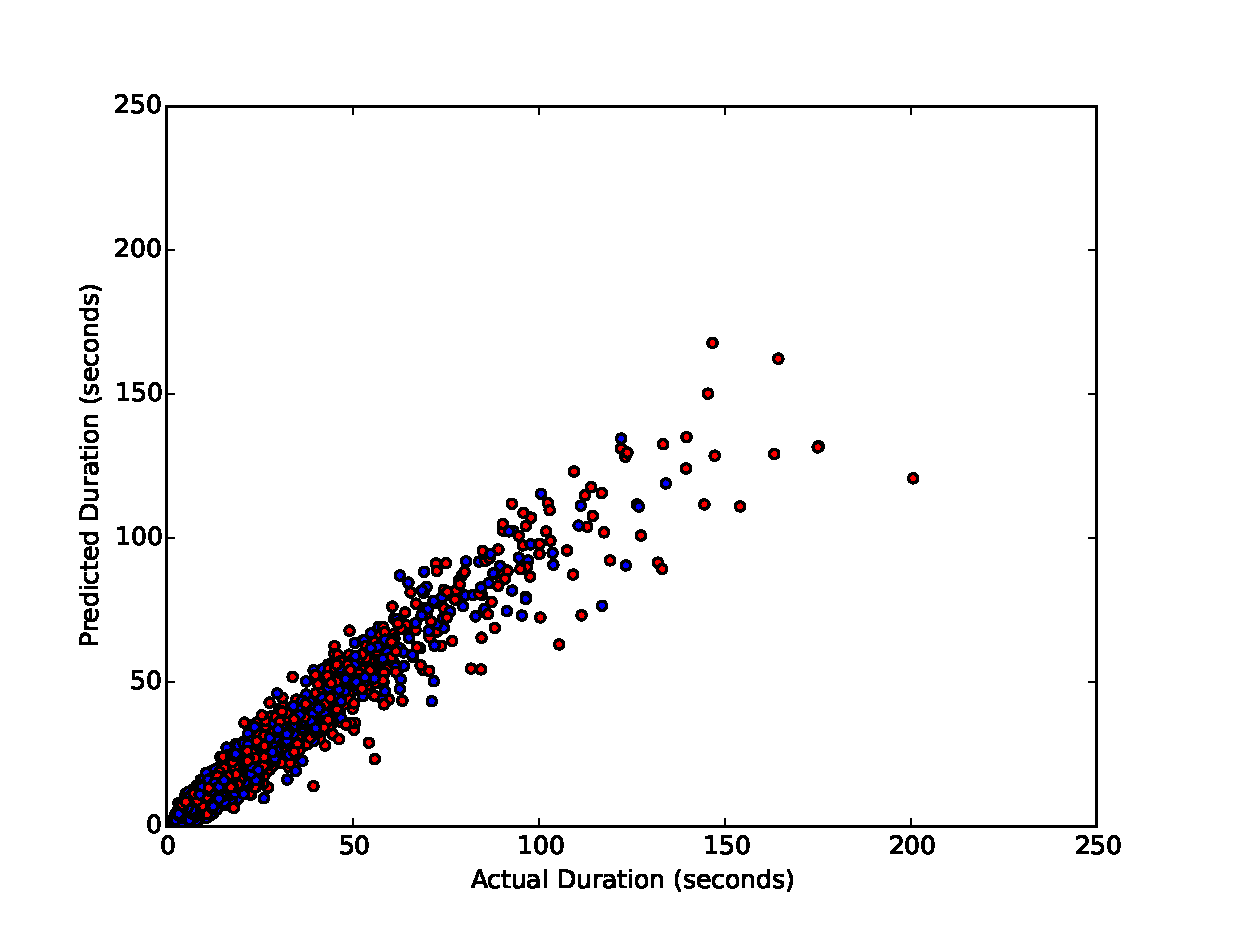
\includegraphics[width=\textwidth]{part11scatter4mer}

$r^2=0.94$


        \newpage
        \subsection*{5mer Model}
        \begin{wrapfigure}{R}{2in}
        \vspace{-50pt}
        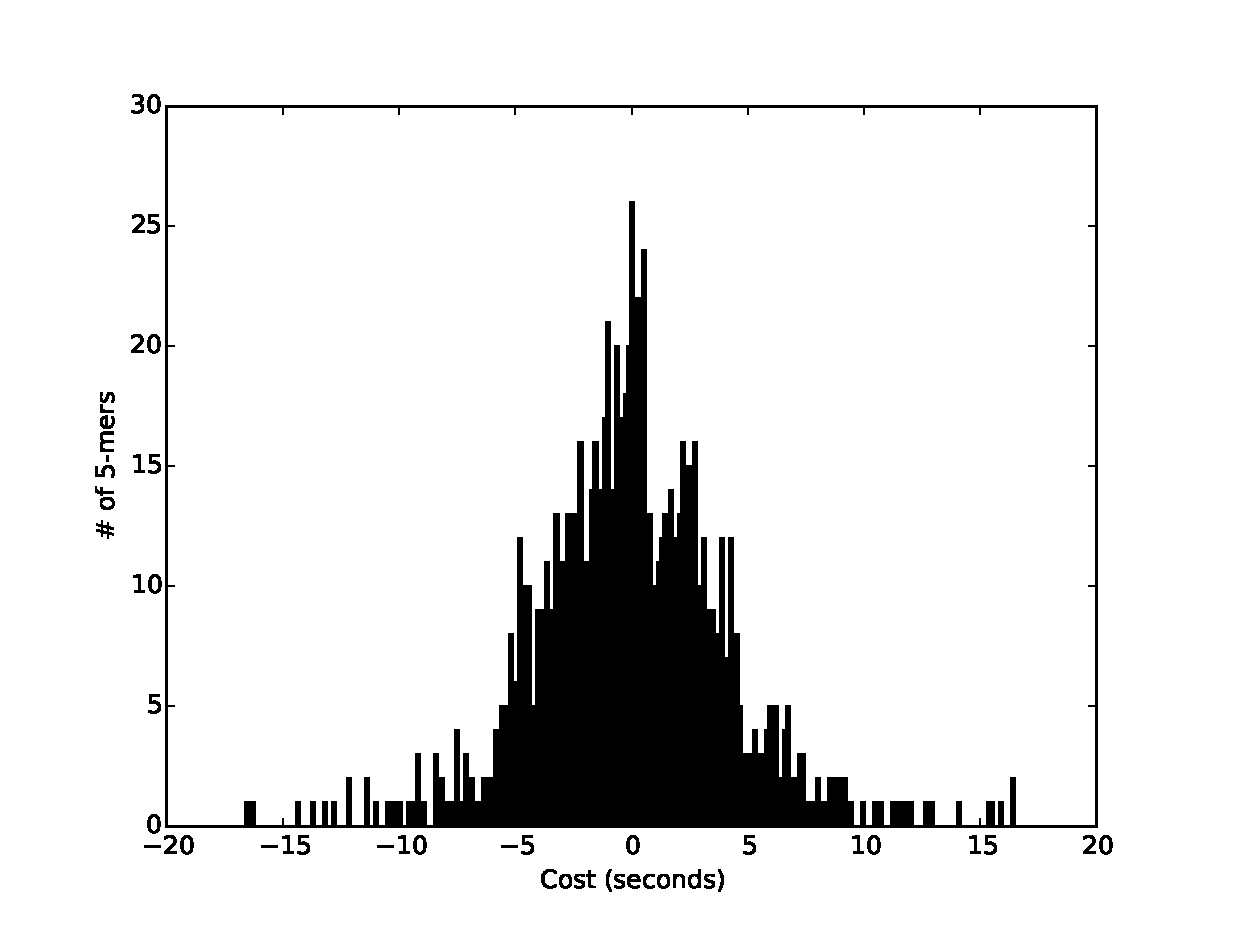
\includegraphics[width=3in]{part11hist5}
        \vspace{-70pt}
        \end{wrapfigure}
        We can use a model in which each the time to extend by one nucleotide is determined by the 5-mer in the middle of the
        pore.  We can not list all the costs, but here's a histogram:

        \vspace{1.5in}

        And here's the resulting predictions:
        
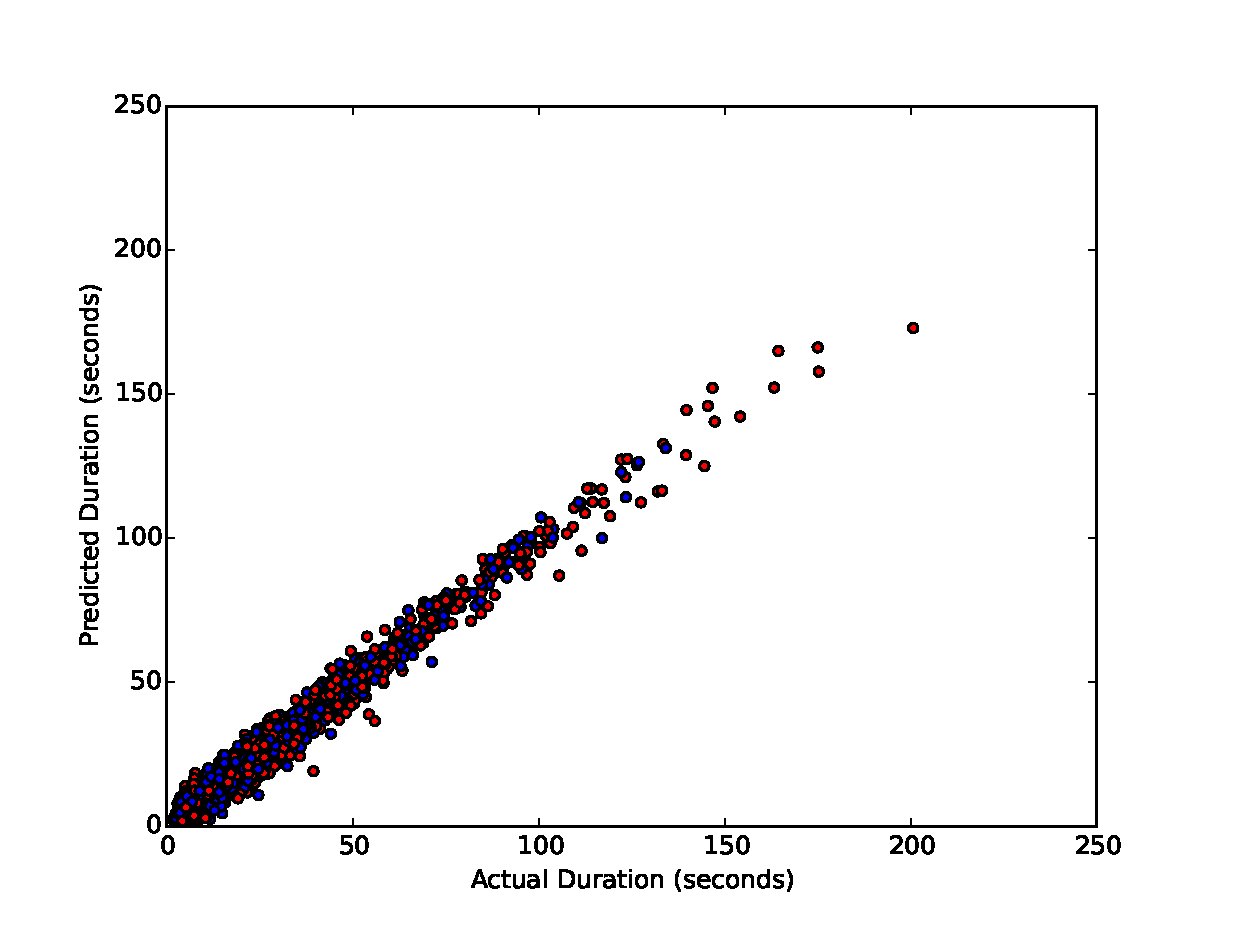
\includegraphics[width=\textwidth]{part11scatter5mer}

$r^2=0.98$



At this point our model has 1024 degrees of freedom for 2162 datapoints, so a good fit may reveal more overfitting than model appropriateness.
\end{document}
